At this stage in the analysis, we are running low on simple cuts which can improve the signal-to-background ratio in the dataset. We must now turn to more complex solutions of separating the signal from potential background seepage. The first method we will use to do this is sPlot\cite{pivk_splot_2005}\footnote{This is stylized as ${}_s\mathcal{P}lot$ in the original paper, but I find this tedious to type and to read.}, a weighting scheme which corrects the na\"ive probabilistic weights one might first think to construct (dubbed ``inPlot'').

We start by developing a model for the signal and background probability distribution functions (PDFs) for a ``discriminating'' variable. We could then weight each event by some normalized probability of it being in the signal distribution rather than the background:

\begin{equation}
  w(x) = \frac{N_S f_S(x)}{N_S f_S(x) + N_B f_B(x)}
  \label{eq:splot:inplot_weights}
\end{equation}
where $x$ is the discriminating variable, $f_S(x)$ and $f_B(x)$ are the corresponding signal and background PDFs, and $N_S$ and $N_B$ are the total number of signal and background events, respectively.

However, as shown by Pivk and Le Diberder\cite{pivk_splot_2005}, we must be careful when using this procedure, as it will only correctly produce signal-isolated plots for ``control'' variables $y$ which are directly correlated with $x$. For the time being, let us assume that this is not the case, and that we wish to use the distribution of some variable which is uncorrelated with the variables we are plotting and analyzing\footnote{We will later see that things are not quite so simple!}. Following the sPlot derivation, we find that, to plot uncorrelated control variables, we must weight our data according to the following scheme:

\begin{equation}
  w(x) = \frac{V_{SS}f_S(x) + V_{SB}f_B(x)}{N_S f_S(x) + N_B f_B(x)},\quad \text{where } V^{-1}_{ij} = \sum_{x} \frac{f_i(x)f_j(x)}{\left(N_S f_S(x) + N_B f_B(x)\right)^2}
  \label{eq:splot:splot_weights}
\end{equation}

The $V^{-1}$ matrix can also be understood as the covariance matrix between the free parameters $N_S$ and $N_B$ in the fit of the signal-background mixture, $V^{-1}_{ij} = -N\pdv[2]{\ln\mathcal{L}}{N_i}{N_j}$, although there is reason to believe this will lead to less accurate results than the manual calculation in \Cref{eq:splot:splot-weights}\cite{dembinski_custom_2022}.

Now that we have a method of assigning weights, we must pick the discriminating variable. Typically, these weighting methods work well on the classic ``bump-on-a-background'' distributions, but because the mass of the kaons is constrained in the kinematic fit, the fitted mass of each kaon is just a $\delta$-function and combination of measured masses for each $\pi^+\pi^-$ pair will yield a Normal distribution with little to no apparent background (by construction). We must be a bit more clever in determining a discriminating variable! By examining the BGGEN analysis done in {\color{red}[TODO: PREVIOUS SECTION]}, we can see that most likely sources of background arise when the intermediate kaons are missing from the reaction: $\gamma p \to 4\pi p$. This reaction shares the $K_SK_S$ final state exactly, so pairs of pions which look close enough to kaons will be almost indistinguishable in the data. However, they differ in one key way, namely that the $K_S$ intermediate contains a strange quark while the $\pi^+\pi^-$ decay state does not, so such a decay must occur via the weak interaction, which is notably slower than the strong interaction which would produce pion pairs with no intermediate kaon. In other words, while the signal's rest-frame lifetime distribution should have an exponential slope near the $K_S$ lifetime, the background would theoretically have nearly zero rest-frame lifetime for every event, or a much smaller exponential slope in practice.

Therefore, we will begin by generating both a signal and background dataset in Monte Carlo. We then interpret both datasets as if they were our desired channel by running them through the GlueX reconstruction and reaction filter, as well as all of our selections up to this point. We can then fit the rest-frame lifetime of each dataset to an exponential model,

\begin{equation}
  f(t) = \lambda \exp{-\lambda t}
  \label{eq:splot:exponential}
\end{equation}
where $\lambda \equiv 1/\tau$, the lifetime of the kaon in question. Since we have two independently decaying kaons, we should really form a joint distribution for both, where we will assume each kaon has the same average lifetime:
\begin{equation}
  f(t_1, t_2) = \lambda^2 \exp{-\lambda t_1}\exp{-\lambda t_2}
  \label{eq:splot:exponential_joint}
\end{equation}
Both the signal and background distributions can be modeled in this way, giving us only two free parameters, $\lambda_S$ and $\lambda_B$ for the signal and background respectively, to fit (see \Cref{fig:mc_f18_splot_fit} for an example of these fits).

\begin{figure}
  \begin{center}
    \begin{subfigure}[b]{.8\columnwidth}
      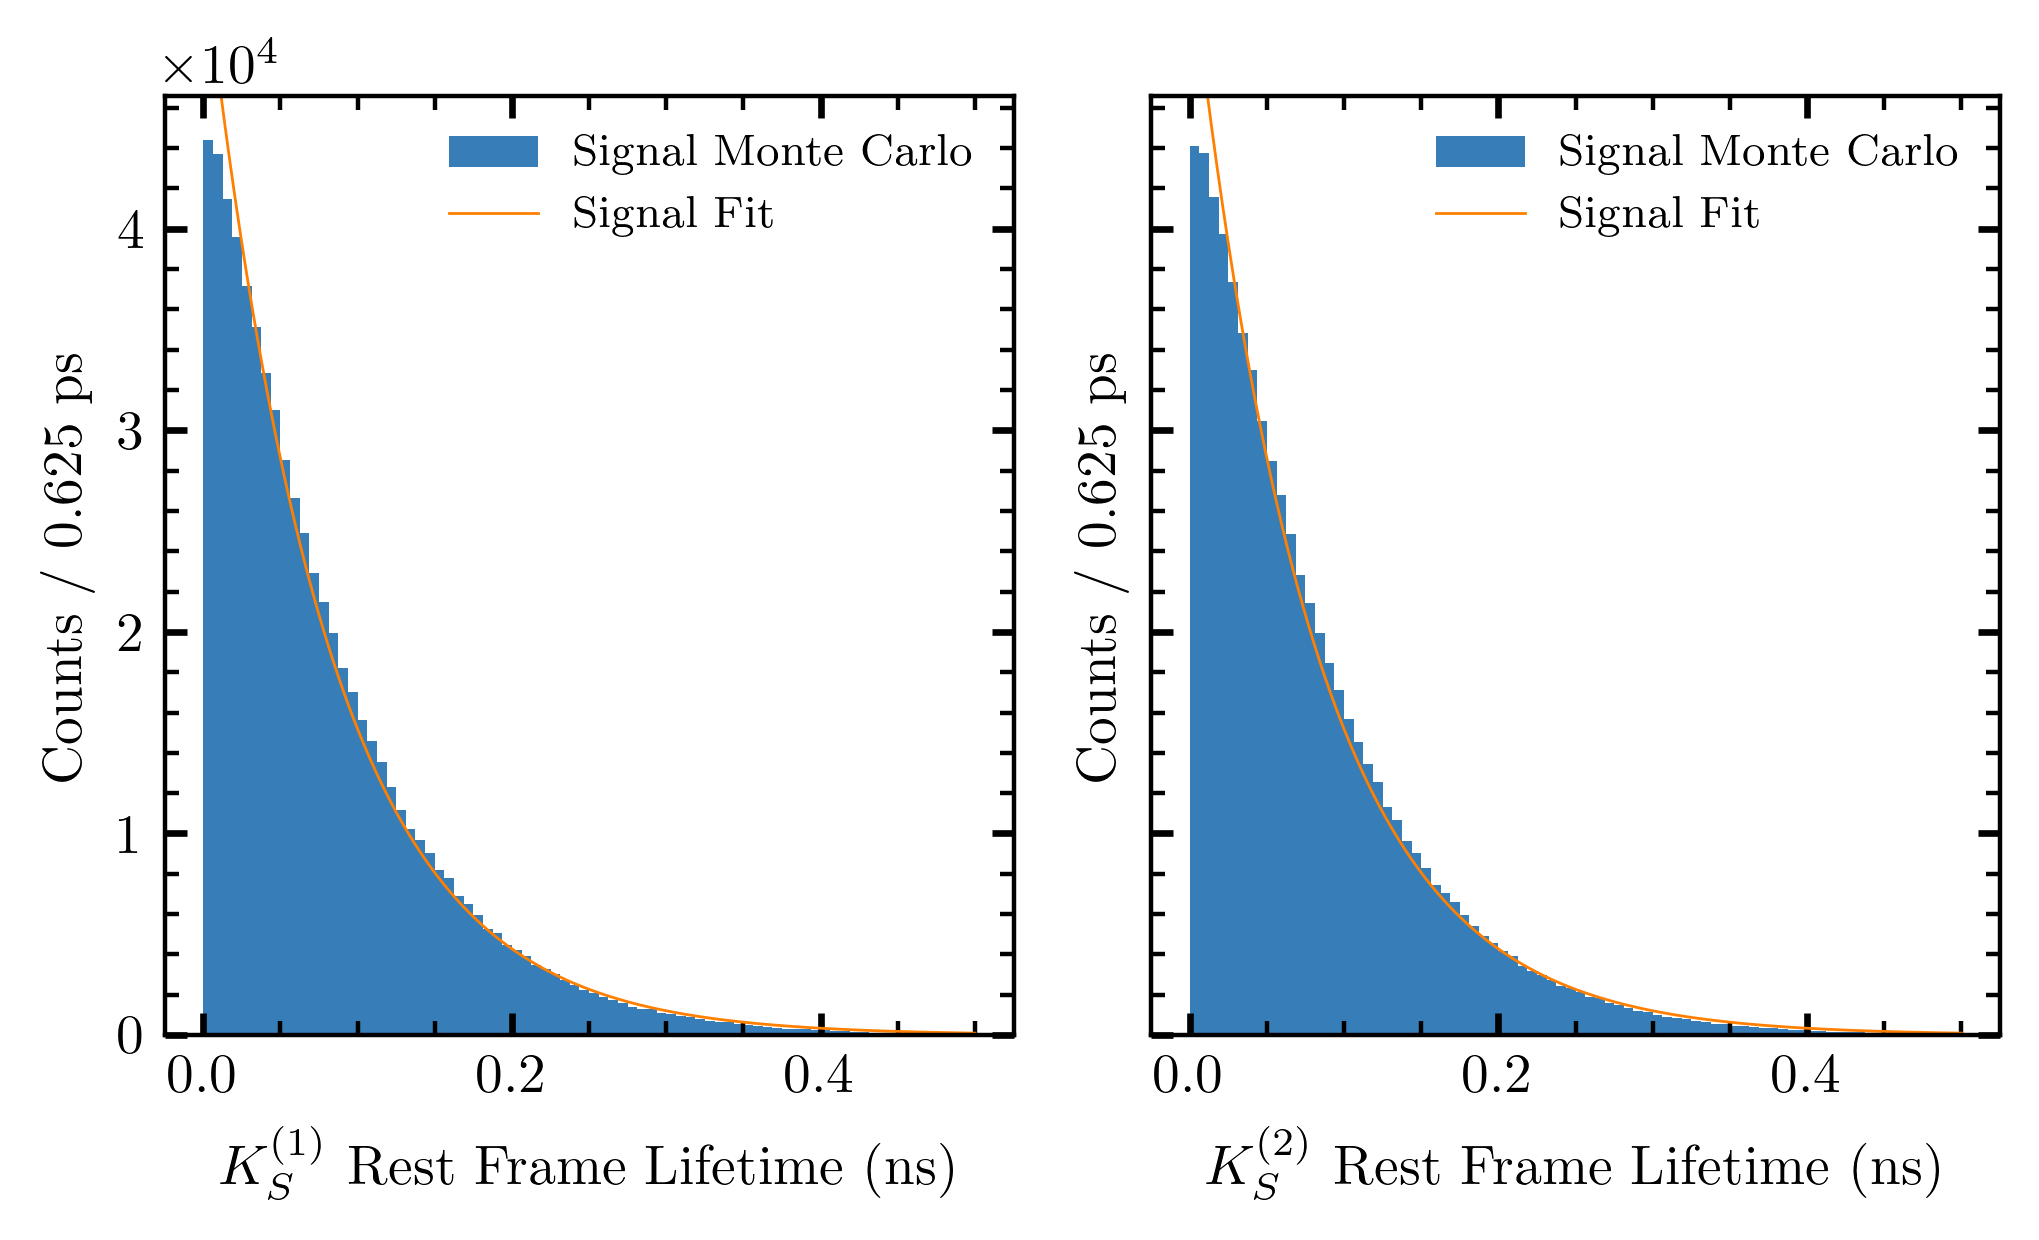
\includegraphics[width=1\linewidth]{figures/sPlot_fit_accmc_F18_fiducial@accidentals@chisqndf-4.png}
      \caption{}
      \label{fig:mc_f18_splot_fit:a}
    \end{subfigure}
    \begin{subfigure}[b]{.8\columnwidth}
      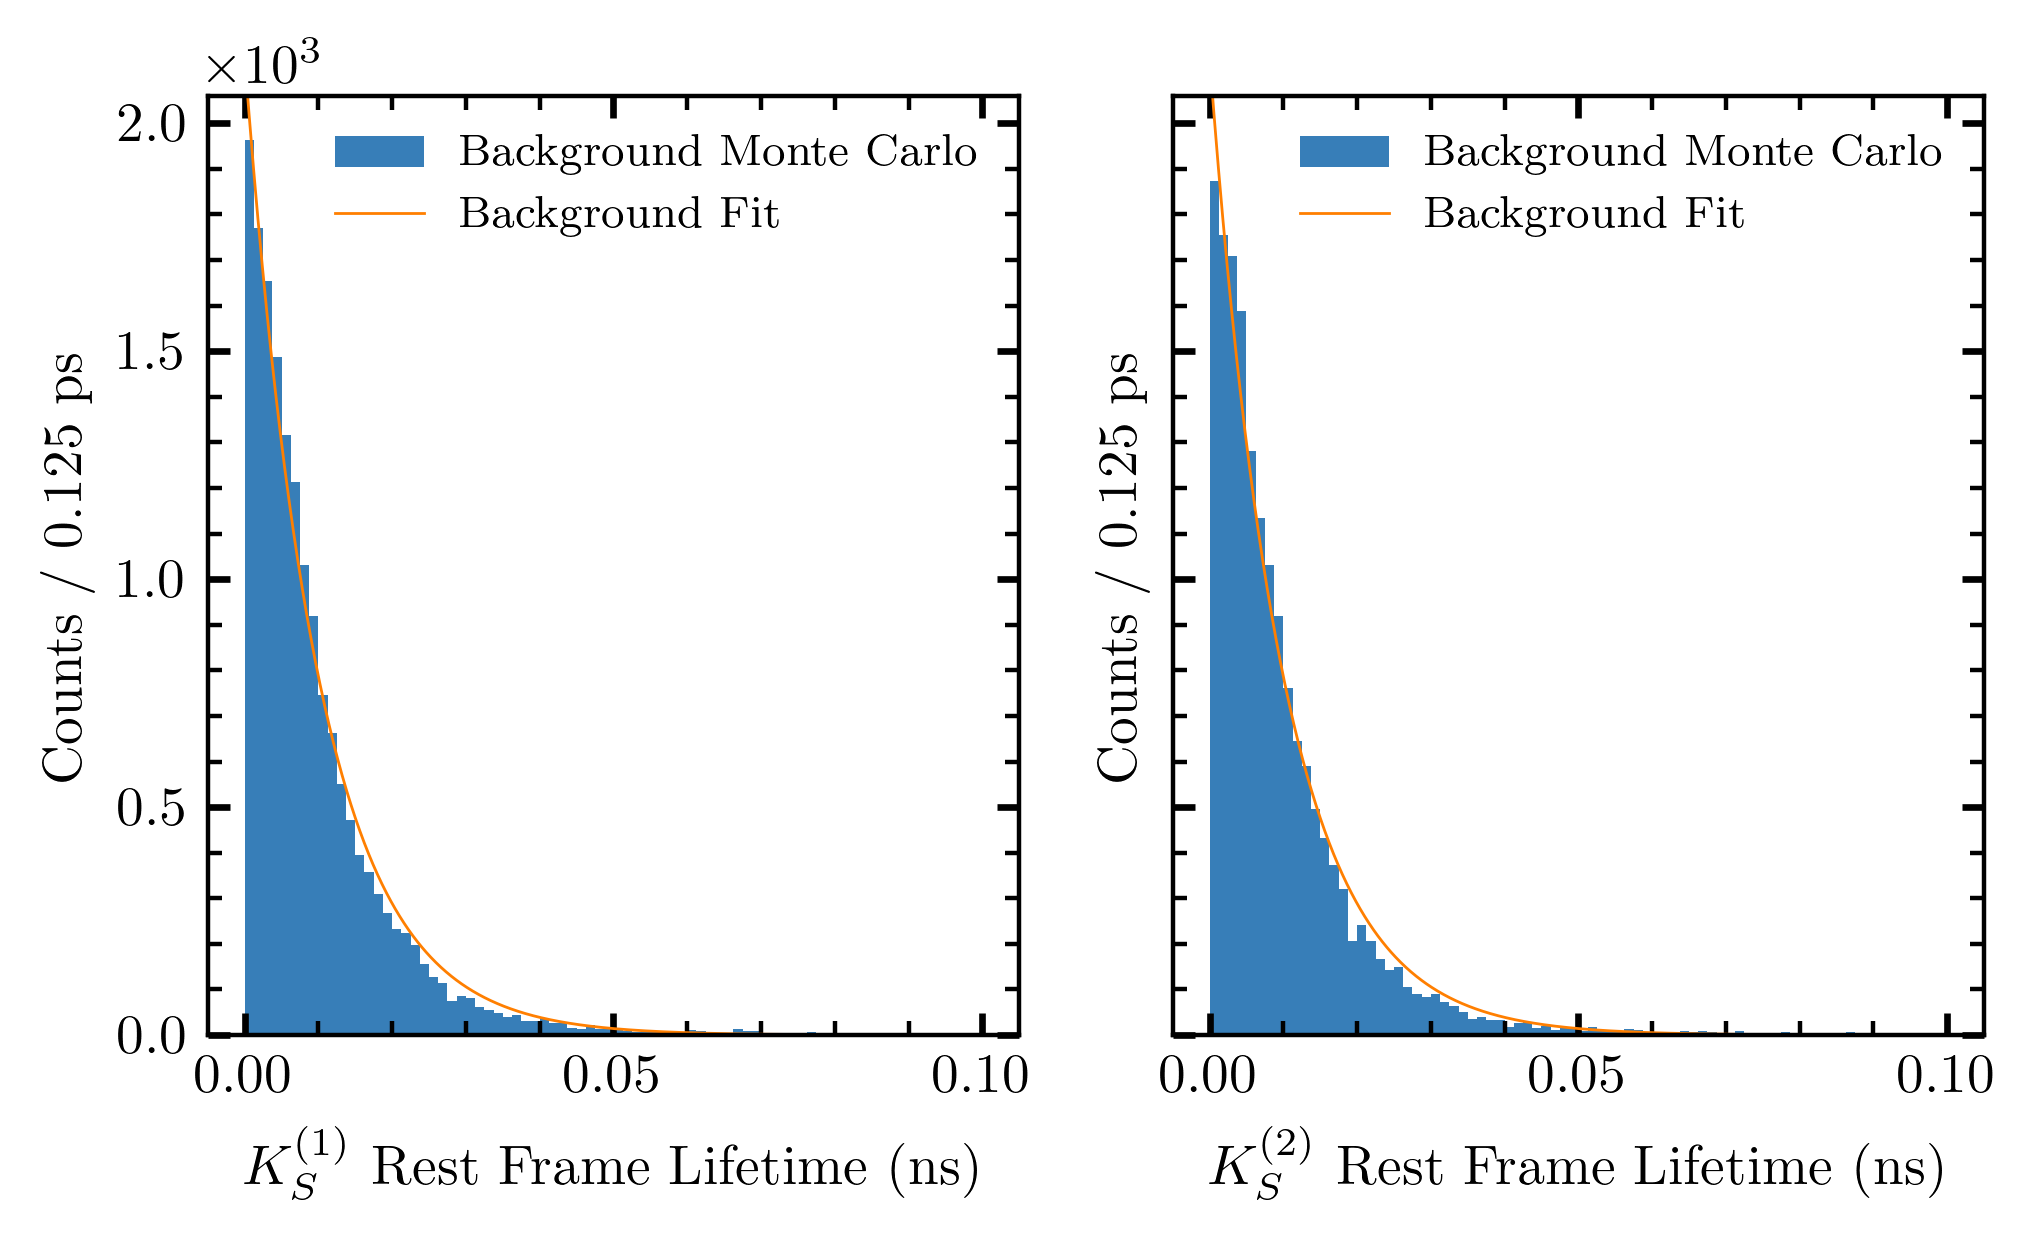
\includegraphics[width=1\linewidth]{figures/sPlot_fit_4pi_F18_fiducial@accidentals@chisqndf-4.png}
      \caption{}
      \label{fig:mc_f18_splot_fit:b}
    \end{subfigure}
  \end{center}
  \caption{(a) Fit of an exponential product model to signal Monte Carlo generated using the F18 beam configuration. (b) The same fit as in (a), but over background Monte Carlo.{\color{red}TODO: zoom axis to 0.2 and plot signal MC as inset}}\label{fig:mc_f18_splot_fit}
\end{figure}


Once we obtain nominal values for $\lambda_S$ and $\lambda_B$ from fits over the signal and background Monte Carlo, we can fix the exponential slopes to the fit values and perform a new fit to our real data with a mixture model (see \Cref{fig:data_f18_splot_fit}):
\begin{equation}
  f(t_1, t_2) = z \lambda_S^2\exp{-\lambda_S t_1}\exp{-\lambda_S t_2} + (1-z) \lambda_B^2\exp{-\lambda_B t_1}\exp{-\lambda_B t_2}
  \label{eq:splot:mixture}
\end{equation}
\begin{figure}
  \begin{center}
    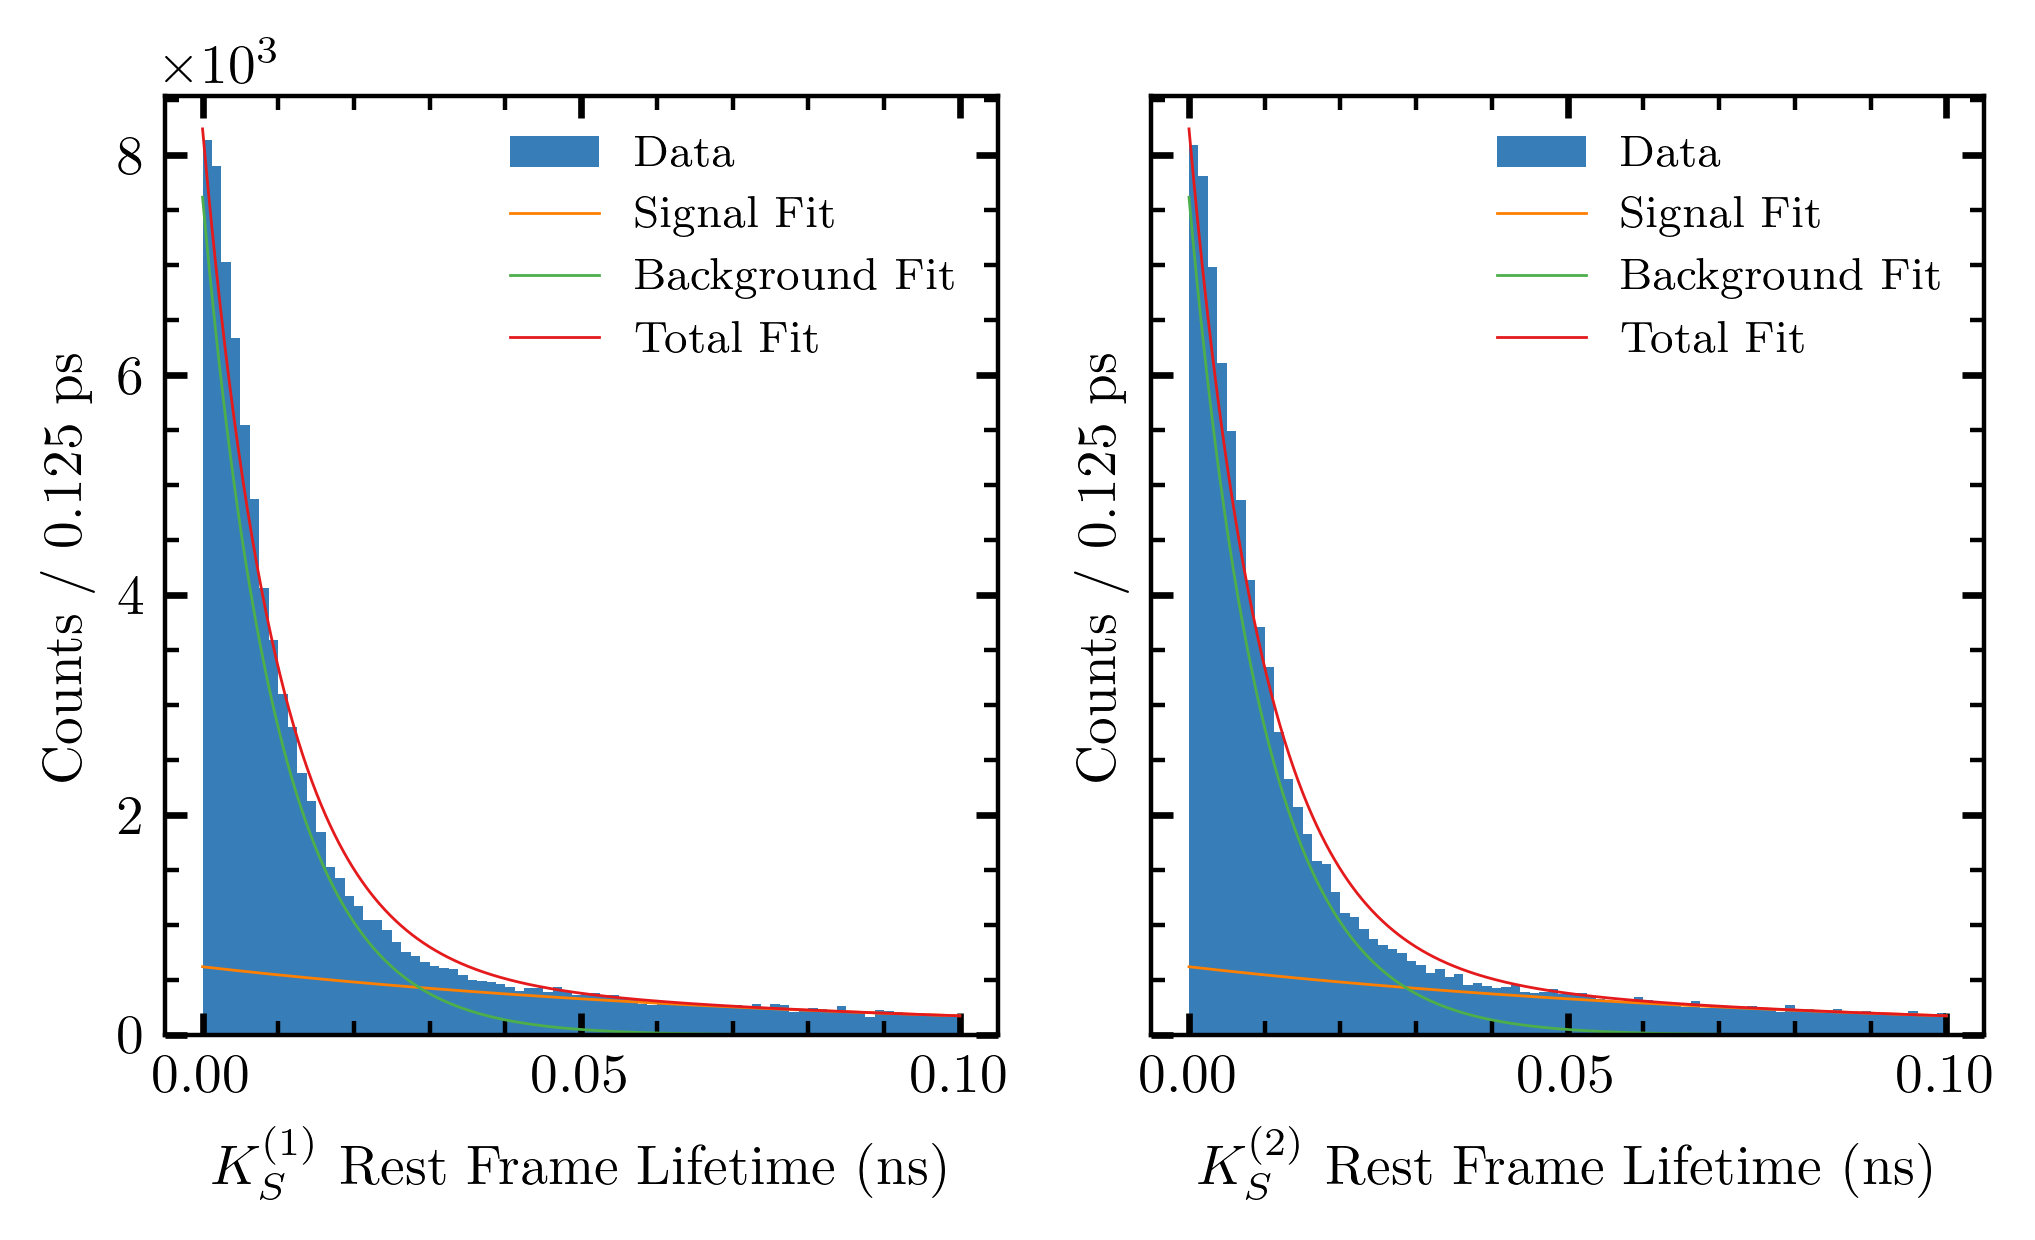
\includegraphics[width=.8\columnwidth]{figures/sPlot_fit_data_F18_fiducial@accidentals@chisqndf-4}
  \end{center}
  \caption{Fit of \Cref{eq:splot:mixture} to data from the F18 run period. True kaon events are prominent in the tail of the distribution, which does not appear in background Monte Carlo samples (\Cref{fig:mc_f18_splot_fit:b}){\color{red}TODO: zoom axis to 0.2}}\label{fig:data_f18_splot_fit}
\end{figure}

In the fit to data, only the fraction of signal to background, $z$, is floating. From its fit value, we can determine values of $N_S$ and $N_B$ to use in \Cref{eq:splot:splot_weights} and complete the weighting procedure.
